% Options for packages loaded elsewhere
\PassOptionsToPackage{unicode}{hyperref}
\PassOptionsToPackage{hyphens}{url}
%
\documentclass[
]{article}
\usepackage{amsmath,amssymb}
\usepackage{lmodern}
\usepackage{iftex}
\ifPDFTeX
  \usepackage[T1]{fontenc}
  \usepackage[utf8]{inputenc}
  \usepackage{textcomp} % provide euro and other symbols
\else % if luatex or xetex
  \usepackage{unicode-math}
  \defaultfontfeatures{Scale=MatchLowercase}
  \defaultfontfeatures[\rmfamily]{Ligatures=TeX,Scale=1}
\fi
% Use upquote if available, for straight quotes in verbatim environments
\IfFileExists{upquote.sty}{\usepackage{upquote}}{}
\IfFileExists{microtype.sty}{% use microtype if available
  \usepackage[]{microtype}
  \UseMicrotypeSet[protrusion]{basicmath} % disable protrusion for tt fonts
}{}
\makeatletter
\@ifundefined{KOMAClassName}{% if non-KOMA class
  \IfFileExists{parskip.sty}{%
    \usepackage{parskip}
  }{% else
    \setlength{\parindent}{0pt}
    \setlength{\parskip}{6pt plus 2pt minus 1pt}}
}{% if KOMA class
  \KOMAoptions{parskip=half}}
\makeatother
\usepackage{xcolor}
\usepackage[margin=1in]{geometry}
\usepackage{longtable,booktabs,array}
\usepackage{calc} % for calculating minipage widths
% Correct order of tables after \paragraph or \subparagraph
\usepackage{etoolbox}
\makeatletter
\patchcmd\longtable{\par}{\if@noskipsec\mbox{}\fi\par}{}{}
\makeatother
% Allow footnotes in longtable head/foot
\IfFileExists{footnotehyper.sty}{\usepackage{footnotehyper}}{\usepackage{footnote}}
\makesavenoteenv{longtable}
\usepackage{graphicx}
\makeatletter
\def\maxwidth{\ifdim\Gin@nat@width>\linewidth\linewidth\else\Gin@nat@width\fi}
\def\maxheight{\ifdim\Gin@nat@height>\textheight\textheight\else\Gin@nat@height\fi}
\makeatother
% Scale images if necessary, so that they will not overflow the page
% margins by default, and it is still possible to overwrite the defaults
% using explicit options in \includegraphics[width, height, ...]{}
\setkeys{Gin}{width=\maxwidth,height=\maxheight,keepaspectratio}
% Set default figure placement to htbp
\makeatletter
\def\fps@figure{htbp}
\makeatother
\setlength{\emergencystretch}{3em} % prevent overfull lines
\providecommand{\tightlist}{%
  \setlength{\itemsep}{0pt}\setlength{\parskip}{0pt}}
\setcounter{secnumdepth}{-\maxdimen} % remove section numbering
\newlength{\cslhangindent}
\setlength{\cslhangindent}{1.5em}
\newlength{\csllabelwidth}
\setlength{\csllabelwidth}{3em}
\newlength{\cslentryspacingunit} % times entry-spacing
\setlength{\cslentryspacingunit}{\parskip}
\newenvironment{CSLReferences}[2] % #1 hanging-ident, #2 entry spacing
 {% don't indent paragraphs
  \setlength{\parindent}{0pt}
  % turn on hanging indent if param 1 is 1
  \ifodd #1
  \let\oldpar\par
  \def\par{\hangindent=\cslhangindent\oldpar}
  \fi
  % set entry spacing
  \setlength{\parskip}{#2\cslentryspacingunit}
 }%
 {}
\usepackage{calc}
\newcommand{\CSLBlock}[1]{#1\hfill\break}
\newcommand{\CSLLeftMargin}[1]{\parbox[t]{\csllabelwidth}{#1}}
\newcommand{\CSLRightInline}[1]{\parbox[t]{\linewidth - \csllabelwidth}{#1}\break}
\newcommand{\CSLIndent}[1]{\hspace{\cslhangindent}#1}
\usepackage{newunicodechar}
\newunicodechar{Δ}{\ensuremath{\Delta}}
\newunicodechar{ ̂}{\ensuremath{\hat}}

\ifLuaTeX
  \usepackage{selnolig}  % disable illegal ligatures
\fi
\IfFileExists{bookmark.sty}{\usepackage{bookmark}}{\usepackage{hyperref}}
\IfFileExists{xurl.sty}{\usepackage{xurl}}{} % add URL line breaks if available
\urlstyle{same} % disable monospaced font for URLs
\hypersetup{
  pdftitle={Supplementary material for `Parental care drives the evolution of reproductive accessory glands in ray-finned fishes'},
  hidelinks,
  pdfcreator={LaTeX via pandoc}}

\title{Supplementary material for `Parental care drives the evolution of
reproductive accessory glands in ray-finned fishes'}
\author{}
\date{\vspace{-2.5em}30 November 2022}

\begin{document}
\maketitle

{
\setcounter{tocdepth}{2}
\tableofcontents
}
\hypertarget{descriptive-statistics}{%
\section{Descriptive statistics}\label{descriptive-statistics}}

\hypertarget{data}{%
\subsection{Data}\label{data}}

\begin{figure}
\centering
\includegraphics{ag_supp_files/figure-latex/barchart-1.pdf}
\caption{Numbers of species with each set of traits (\texttt{0} =
absent, \texttt{1} = present, \texttt{?} = unknown; \texttt{pc} = male
parental care; \texttt{sc} = sperm competition (i.e.~group spawning or
ARTs); \texttt{ag} = accessory glands), depending on whether we use the
partial (but fully genetically resolved) tree (\texttt{fishphylo}) or
the imputed trees from Rabosky et al. (2018) (\texttt{treeblock}).}
\end{figure}

The phylogenies in the treeblock are generated according to an
imputation scheme described in Rabosky et al. (2018). We generated 100
stochastic character maps for each of 100 trees; the figure shows the
average number of gains and losses per tree (i.e., average gains/losses
across the stochastic character maps for each tree).

\begin{verbatim}
## Warning: run figures.R?
\end{verbatim}

\begin{figure}
\centering
\includegraphics{ag_supp_files/figure-latex/densitree-1.png}
\caption{densitree-style (Bouckaert 2010) mapping of tree
blocks/phylogenetic uncertainty}
\end{figure}

\hypertarget{parameter-definitions}{%
\section{Parameter definitions}\label{parameter-definitions}}

\hypertarget{transition-matrices}{%
\subsection{Transition matrices}\label{transition-matrices}}

As described in the main text, a continuous-time stochastic process for
three binary traits has a total of 24 possible transitions where a
single one of the three states changes. The figure below shows the full
and reduced transition matrices. In the axis tick labels,
\texttt{ag0\_pc0\_sc1} (for example) refers to the state without AGs
(\texttt{ag0}), without male care (\texttt{pc0}), and with group
spawning (\texttt{sc1}, loosely ``sperm competition
present''\footnote{Hereafter we refer to pair spawning as ``sperm
  competition absent'' (\texttt{sc0}) and group spawning as ``sperm
  competition present'' (\texttt{sc1}), recognizing that this is an
  oversimplification.}). Parameter 1 quantifies the log-hazard of a
switch to pair spawning in this state (i.e., to \texttt{ag0\_pc0\_sc0}).

The assignment of numbers to rates is arbitrary, numbered in sequence in
column-wise order. Knowing the assignment is only necessary when doing
low-level computations based on the vector of parameters. The take-home
information is which sets of transitions are constrained to be identical
in the reduced model; these rates have the same number . In the reduced
model (righthand plot), transitions that are assumed to have equal rates
- because we assume that all transitions in spawning mode, and all
transitions in male care, are independent of the other states - have the
same ID number. Colours denote the estimated log-hazard for each
parameter when the models are fitted by maximum likelihood. Below, we
denote parameter 1 (in the reduced model, which occupies four different
cells in the transition matrix) as \texttt{sc\_loss}, because it
quantifies the loss rate of sperm competition regardless of the states
of the other traits; we refer to parameter 3 (for example) as
\texttt{loss.ag\_pc0\_sc1}, the loss rate of AGs in the absence of male
care and presence of sperm competition.

\begin{figure}
\centering
\includegraphics{ag_supp_files/figure-latex/image-1.pdf}
\caption{Transition matrix for full and reduced (independent evolution
of spawning mode and male care) models. Colours of grid squares
represent the estimated evolutionary rates (log-hazards) for each
transition. Note that the rates for 24-parameter model are extremely
uncertain; see sensitivity analysis (last section).}
\end{figure}

\hypertarget{transitions}{%
\subsection{Transitions}\label{transitions}}

\begin{figure}
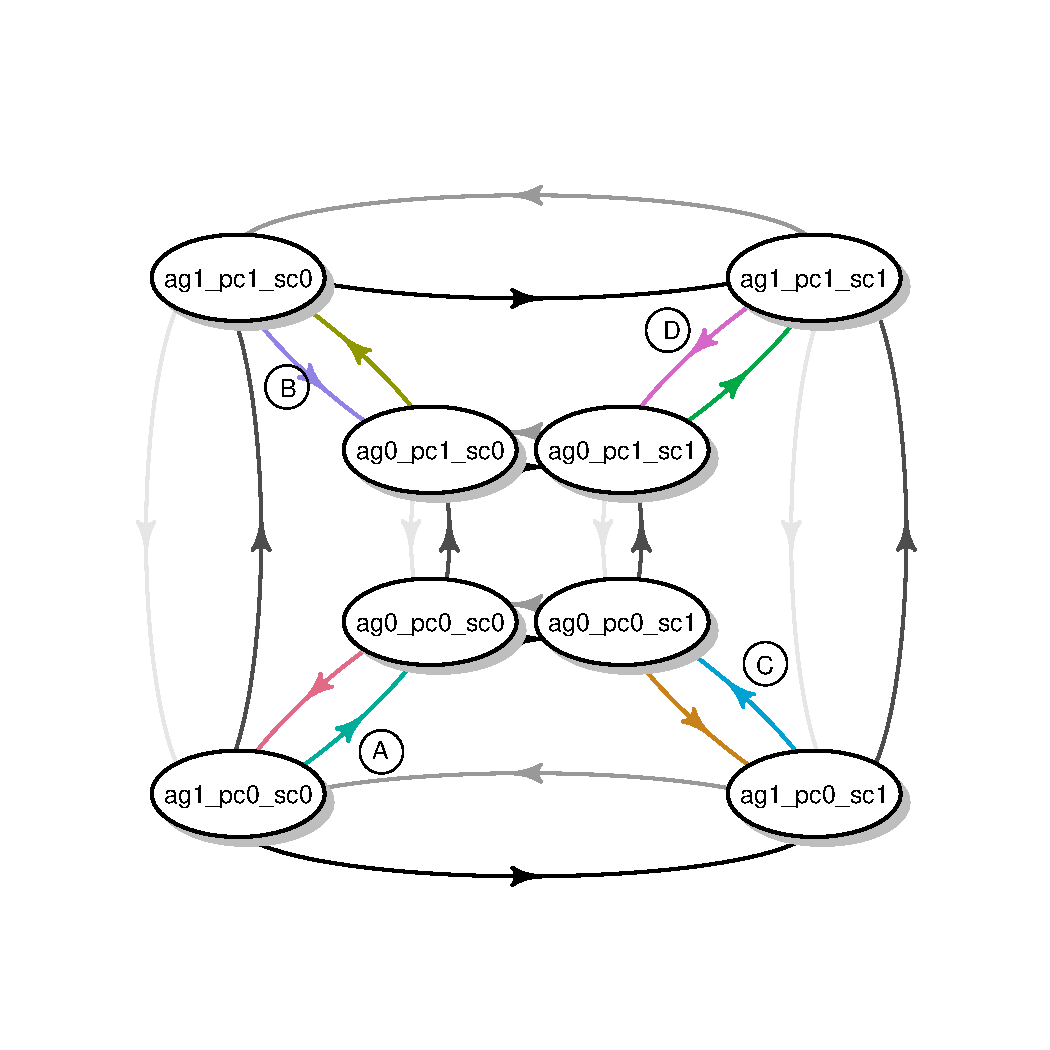
\includegraphics[width=6in,height=6in]{pix/flowfig2} \caption{Transitions for the reduced (12-parameter) model. As in Figure 1 in the main text: Sets of connections drawn with the same colours are constrained to identical evolutionary rates (e.g. light gray downward arrows, representing loss of male parental care – all transitions from “pc1” to the corresponding “pc0” state). Top-bottom and left-right transitions, representing loss/gain of parental care and transitions between pair spawning and group spawning, are assumed to be independent of other trait values. Loss/gain of accessory glands (diagonal arrows), which are our primary interest, are all estimated separately (8 different colours for arrows representing loss/gain of accessory glands under the 4 different combinations of the other two traits, parental  care and spawning mode).}\label{fig:contrast-diag}
\end{figure}

The transitions denoted A-D all represent gains of accessory glands,
under different combinations of male care/spawning mode. Arrows A and B
both represent AG gains in states with pair spawning (\texttt{sc0}); C
and D both represent states in states with group spawning
(\texttt{sc1}). Thus rate(pair) = (rate(A) + rate(B))/2 is the average
rate of AG gain under pair spawning; rate(group) = (rate(C) + rate(D))/2
is the average rate under group spawning; and rate(group)-rate(pair) is
the \emph{contrast}, which we can think of as ``the effect of group vs
pair spawning on the rate of AG gain''. We can similarly compute other
combinations such as rate(no male care) (\texttt{pc0}) = (rate(B) +
rate(D))/2; rate(male care) (\texttt{pc1}) = (rate(A) + rate(C))/2; and
contrast(male care) = rate(male care) - rate(no male care).

\hypertarget{contrast-matrix}{%
\subsection{Contrast matrix}\label{contrast-matrix}}

The \emph{contrast matrix} connects the parameters we estimate
(e.g.~\texttt{loss.ag\_pc0\_sc0}, loss rate of accessory glands when
parental care and sperm competition are both absent) to the biological
effects we are interested in (e.g.~\texttt{pc\_loss}, the effect of
parental care on the loss rate of accessory glands). For example, the
\texttt{intercept\_loss} effect is the (unweighted) average of the four
different loss terms; the \texttt{pc\_loss} effect is the difference
between the average loss rate when male care is present (second row, red
squares) and the average loss rate when male care is absent (second row,
blue squares).

\begin{figure}
\centering
\includegraphics{ag_supp_files/figure-latex/plot-contrast-mat-1.pdf}
\caption{Contrast matrix defining translation from internal rate
parameters (columns, corresponding to transition rates in Figure 1.3) to
meaningful contrasts (see figures below). Gain and loss terms for group
spawning and male care not shown, as these are not translated into
contrasts.}
\end{figure}

Here is an equivalent numeric matrix:

\[
\left[
\begin{array}{rrrrrrrr}
1/4 & 1/4 & 1/4 & 1/4 & . & . & . & . \\
-1/2 & -1/2 & 1/2 & 1/2 & . & . & . & . \\
1/2 & -1/2 & -1/2 & 1/2 & . & . & . & . \\
-1/2 & 1/2 & -1/2 & 1/2 & . & . & . & . \\
. & . & . & . & 1/4 & 1/4 & 1/4 & 1/4 \\
. & . & . & . & -1/2 & 1/2 & -1/2 & 1/2 \\
. & . & . & . & -1/2 & -1/2 & 1/2 & 1/2 \\
. & . & . & . & 1/2 & -1/2 & -1/2 & 1/2 \\
\end{array}
\right]
\]

\hypertarget{priors}{%
\section{Priors}\label{priors}}

Here we illustrate our general strategy for constructing priors: pick
sensible lower and upper ``bounds'' (not really bounds, but values we
would consider extreme) and use a Normal prior on the log-hazard scale
(equivalent to a log-Normal prior on the hazard scale) with a mean
halfway between the lower and upper bounds and a standard deviation
\(\sigma = (\log(\textrm{upper})-\log(\textrm{lower}))/(2 \cdot \textrm{range})\)
In our model we use a range of 3 (i.e.~the lower and upper bounds are at
\(\pm 3 \sigma\)), to denote that the lower and upper bounds we specify
are extreme (99.7\% ranges). The figure below uses range = 2 (which
would correspond to 95.4\% ranges) so the tails are more clearly
visible.

\begin{figure}
\centering
\includegraphics{ag_supp_files/figure-latex/prior-spec-1.pdf}
\caption{Schematic of prior definition in terms of lower and upper tails
of a Gaussian distribution. Left, linear scale; right, log scale}
\end{figure}

By sampling directly from the prior and computing contrasts, we can
confirm that the priors on the contrasts (ratio of AG gain/loss rates
depending on male care and sperm competition) are indeed neutral
(centered at 1.0) and reasonable (95\% confidence intervals extend from
10x slower to 10x faster). The intercept terms for gain and loss
represent the \emph{average} evolutionary rates across all states, and
are measured in units of expected numbers of events across the entire
tree. For example, the prior expected number of gains of AG across the
whole tree is 33.4 (95\% CI: 10.8-105.9).

\begin{figure}
\centering
\includegraphics{ag_supp_files/figure-latex/priorsamp-fig-1.pdf}
\caption{95\% CIs for prior distributions of contrasts}
\end{figure}

\hypertarget{statistical-summaries}{%
\section{Statistical summaries}\label{statistical-summaries}}

This section presents the quantitative results in more detail.

\hypertarget{bayesian}{%
\subsection{Bayesian}\label{bayesian}}

Here are the estimated posterior median and confidence intervals, along
with \(p_\textrm{MCMC}\) (twice the minimum tail probability) and the
``probability of direction'' (\(p_d\)), the probability that the
parameter has the same sign as the median (\(p_d\) is an index of how
clearly the sign of the parameter is known:
\(p_\textrm{MCMC} = 2(1-p_d)\)) (Makowski et al. 2019; Shi and Yin
2021).

\begin{longtable}[]{@{}llrrrrr@{}}
\toprule()
contrast & rate & median & lwr & upr & pMCMC & pd \\
\midrule()
\endhead
intercept & gain & 18.137 & 8.834 & 34.901 & NA & NA \\
pc & gain & 5.755 & 1.352 & 23.492 & 0.019 & 0.991 \\
pcxsc & gain & 0.511 & 0.119 & 2.118 & 0.355 & 0.823 \\
sc & gain & 0.254 & 0.060 & 1.056 & 0.061 & 0.970 \\
intercept & loss & 68.239 & 27.553 & 174.638 & NA & NA \\
pc & loss & 0.966 & 0.133 & 5.667 & 0.970 & 0.515 \\
pcxsc & loss & 0.496 & 0.074 & 2.832 & 0.443 & 0.779 \\
sc & loss & 0.687 & 0.117 & 4.698 & 0.684 & 0.658 \\
\bottomrule()
\end{longtable}

Here are the marginal posterior distributions for all of the contrasts,
including fits to both the full tree-block data set and the subset of
the data that includes only species with genetic data (``fishphylo'').
(The latter is useful for comparison with the MLE results, which cannot
use the Bayesian method of sampling across treeblock phylogenies.) The
treeblock estimates are slightly more precise (i.e.~the confidence
intervals are narrower), as expected since they can make use of a larger
data set. Points show the posterior median, Line ranges represent 95\%
credible intervals.

\begin{verbatim}
## Warning: Computation failed in `stat_summary()`
## Computation failed in `stat_summary()`
## Computation failed in `stat_summary()`
## Computation failed in `stat_summary()`
## Caused by error in `fun.data()`:
## ! The package `Hmisc` is required.
\end{verbatim}

\includegraphics{ag_supp_files/figure-latex/plot-contrasts-1.pdf}

\hypertarget{frequentist}{%
\subsection{Frequentist}\label{frequentist}}

\hypertarget{likelihood-ratio-tests}{%
\subsubsection{Likelihood ratio tests}\label{likelihood-ratio-tests}}

For any pair of \emph{nested} models we can do a likelihood ratio test,
comparing the model fits and number of parameters. We fit restricted
models with AG evolution independent of both sperm competition and male
care (\texttt{indep}); dependent on male care but not sperm competion
(\texttt{pc}); dependent on sperm competition only (\texttt{sc});
depending \emph{additively} on both traits (i.e., the effects of the
trait status on evolutionary rates are added, on the log scale - this
model has 10 parameters); and with an interaction between traits (the
full 12-parameter model that is our primary focus).

Testing (most) nested pairs gives this diagram (we omit the comparison
between \texttt{pcsc} and \texttt{indep}):

\begin{figure}
\centering
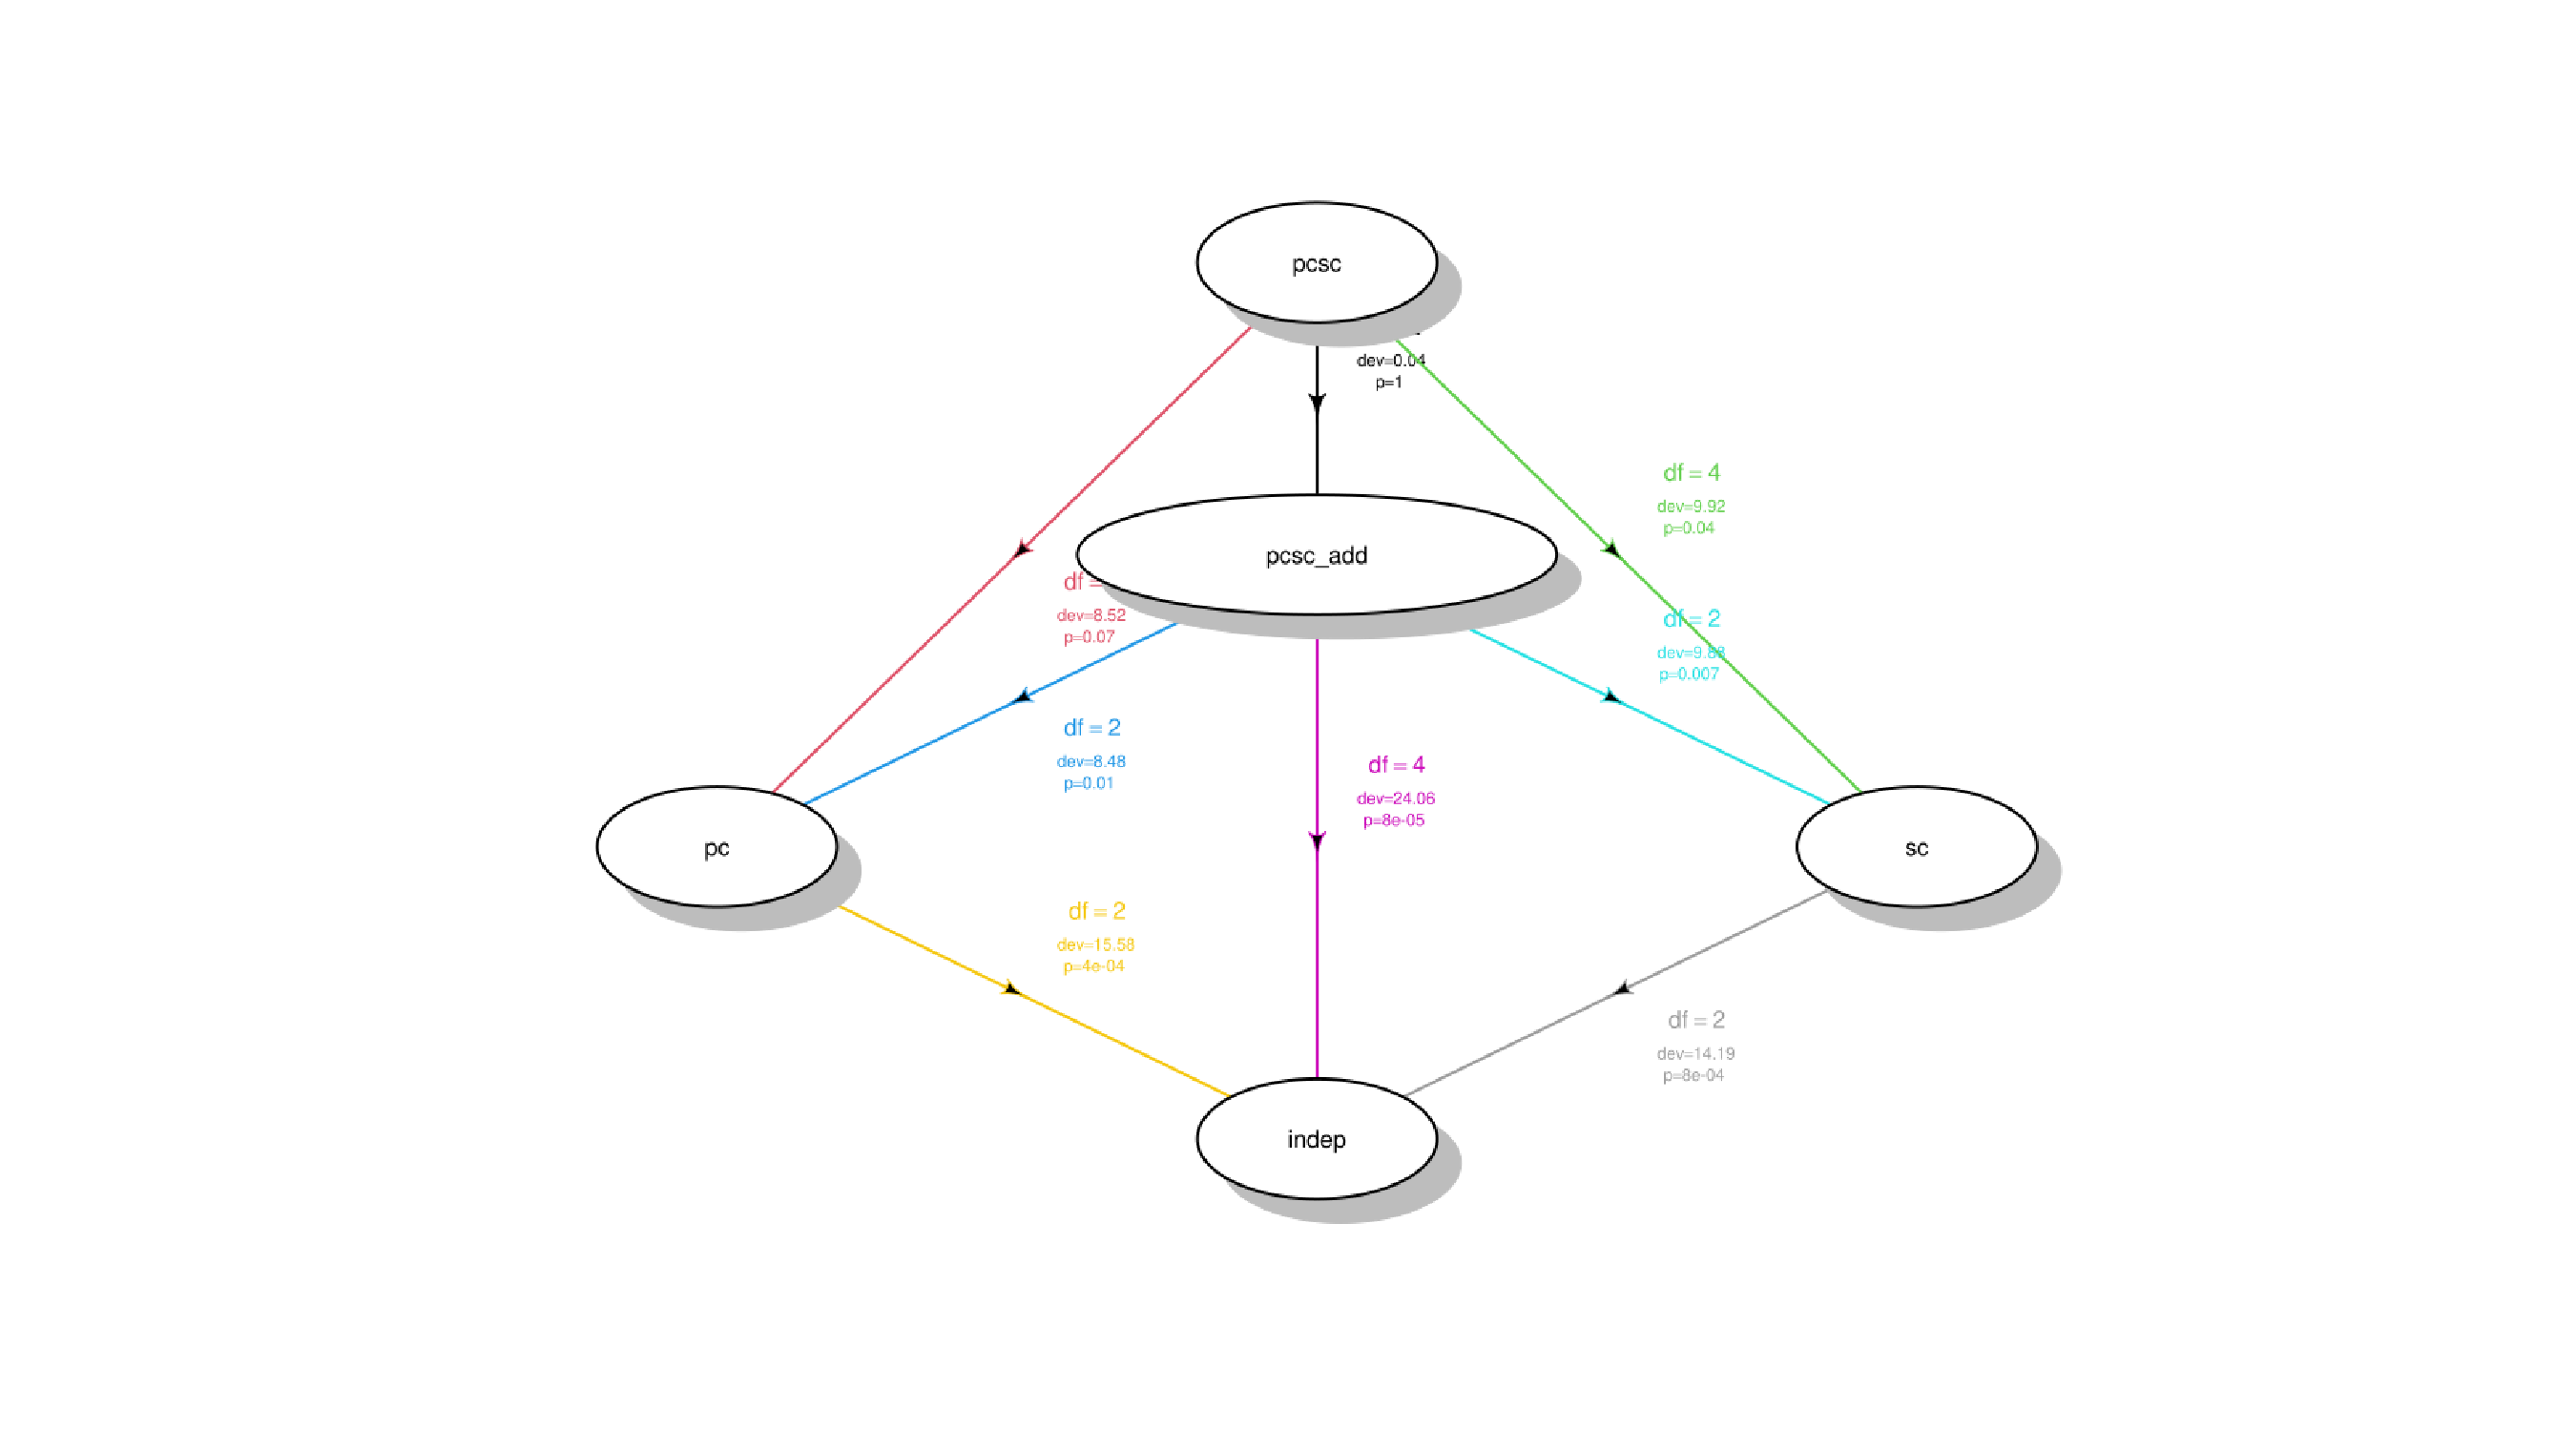
\includegraphics{pix/lrt_comp.pdf}
\caption{likelihood ratio test comparisons}
\end{figure}

The p-values quoted in the paper are from comparing the full model with
interactions to the \texttt{pc} and \texttt{sc} models. These
comparisons are analogous to ``type 3'' tests in ANOVA (Fox and Weisberg
2018), which are the most commonly used approach in the biological
literature. ``Type 2'' tests (as implemented in the \texttt{car} package
for R) instead compare the \emph{additive} model to the models with only
one main effect: these tests suggest that the effects of both sperm
competition and male care are statistically significant, although the
evidence for the effect of male care is still stronger.

\begin{longtable}[]{@{}llrrr@{}}
\toprule()
& desc & ddf & ddev & pval \\
\midrule()
\endhead
pcsc & interaction & 2 & 0.040 & 0.980 \\
sc3 & sc (type III) & 4 & 8.519 & 0.074 \\
sc2 & sc (type II) & 2 & 8.479 & 0.014 \\
pc3 & pc (type III) & 4 & 9.918 & 0.042 \\
pc2 & pc (type II) & 2 & 9.878 & 0.007 \\
\bottomrule()
\end{longtable}

(\texttt{ddf}: difference in number of parameters between models;
\texttt{ddev}: change in deviance (\(-2 \log(L)\)); \texttt{pval}:
likelihood ratio test p-value)

\hypertarget{parameter-estimatescis}{%
\subsubsection{Parameter estimates/CIs}\label{parameter-estimatescis}}

We can look at the parameter estimates from maximum likelihood fits,
although most of the confidence intervals of the unregularized fits are
undetermined because of the failure of the Wald estimates. All
confidence intervals more extreme than \(\exp(\pm 20)\) are set to 0 or
\(\infty\).

Profile confidence intervals could give slightly better results, but
these turds may be not worth polishing very much \ldots{}

\begin{longtable}[]{@{}llrrr@{}}
\toprule()
method & term & estimate & lwr & upr \\
\midrule()
\endhead
pcsc & pc\_loss & 0.273 & 0.000 & Inf \\
pcsc & sc\_loss & 3.668 & 0.000 & Inf \\
pcsc & pcxsc\_loss & 0.000 & 0.000 & Inf \\
pcsc & pc\_gain & 2.664 & 0.000 & Inf \\
pcsc & sc\_gain & 0.003 & 0.000 & Inf \\
pcsc & pcxsc\_gain & 0.375 & 0.000 & Inf \\
pcsc\_prior & pc\_loss & 0.973 & 0.170 & 5.550 \\
pcsc\_prior & sc\_loss & 0.654 & 0.117 & 3.652 \\
pcsc\_prior & pcxsc\_loss & 0.612 & 0.109 & 3.452 \\
pcsc\_prior & pc\_gain & 4.156 & 1.075 & 16.069 \\
pcsc\_prior & sc\_gain & 0.297 & 0.075 & 1.177 \\
pcsc\_prior & pcxsc\_gain & 0.729 & 0.181 & 2.940 \\
pcsc\_add & pc\_loss & 10000.000 & 0.000 & Inf \\
pcsc\_add & sc\_loss & 0.001 & 0.000 & Inf \\
pcsc\_add & pc\_gain & 8.352 & 2.030 & 34.358 \\
pcsc\_add & sc\_gain & 0.001 & 0.000 & Inf \\
\bottomrule()
\end{longtable}

\hypertarget{information-theoretic-comparisons}{%
\subsubsection{Information-theoretic
comparisons}\label{information-theoretic-comparisons}}

Alternatively, we can make comparisons based on information-theoretic
criteria such as AICc, AIC, or BIC. These three criteria differ in the
kind and strength of penalty that they use to avoid overly complex
models. Researchers choose different criteria depending on their goals -
strictly speaking AIC and its variants are for maximizing predictive
accuracy while BIC is for choosing among hypotheses. AICc is often
recommended for analyses where \(n<40\). Using AICc presents a
challenge: for this data set (a phylogeny of 607 species with
approximately 20 independent origins of accessory glands), it is
difficult to quantify the \emph{effective} number of observations (the
\(n\) in the rule of thumb above, and in the formula for the AICc, is
based on a simpler data format where we can assume that every
observation is independent). We chose \(n=30\) for this comparison, as a
guess at the effective sample size (larger \(n\) will tend to select
larger models as better).

Negative log-likelihood, which measures the unpenalized goodness-of-fit,
is included for completeness/comparison.

\begin{longtable}[]{@{}lrrrrr@{}}
\toprule()
& df & ΔAICc & ΔAIC & ΔBIC & ΔnegLL \\
\midrule()
\endhead
AG dep only on PC & 8 & 0.00 & 4.48 & 1.68 & 4.26 \\
AG dep on PC, SC additively & 10 & 0.24 & 0.00 & 0.00 & 0.02 \\
AG dep only on SC & 8 & 1.40 & 5.88 & 3.08 & 4.96 \\
AG evol indep of PC, SC & 6 & 8.38 & 16.06 & 10.46 & 12.05 \\
AG dep on PC, SC \& interaction & 12 & 10.98 & 3.96 & 6.76 & 0.00 \\
\bottomrule()
\end{longtable}

As stated in the main text, we can see that AICc gives similar
conclusions to the Bayesian and likelihood-ratio-test analyses: the best
model has AG evolution depending on male care only, followed closely by
the additive model, and fairly closely by sperm competition only (models
with \(\Delta\) AICc \textless{} 2 are usually interpreted as ``roughly
equivalent''). In contrast, using AIC selects the additive model as
best, and considerably better than the single-factor models. BIC, which
like AICc is generally more conservative than AIC, also selects the
additive model as best, similar (\(\Delta\) BIC \textless{} 2) to the
male-care-only model.

\hypertarget{sensitivity-analyses}{%
\section{Sensitivity analyses}\label{sensitivity-analyses}}

We performed a range of different analyses to test the sensitivity of
our conclusions to technical choices, and to explore the difference
between frequentist (maximum likelihood estimate = MLE), constrained
frequentist (maximum \emph{a posteriori} = MAP), and full Bayesian
(MCMC) fitting methods.

\begin{itemize}
\tightlist
\item
  \texttt{mcmc\_tb}: Bayesian MCMC using neutral priors on the
  transition rates and biologically informed priors on the gain/loss
  rates; this is the primary model presented in the main text
\item
  \texttt{mcmc\_0}: as \texttt{mcmc\_tb}, but using only the completely
  resolved phylogeny (i.e., only including species for which genetic
  data is available)
\item
  \texttt{mcmc\_tb\_nogainloss}: as \texttt{mcmc\_tb}, but using only
  the priors on the transition rates, omitting the priors on the
  gain/loss rates
\item
  \texttt{full}: a model estimating all 24 transition rates,
  i.e.~allowing for the rates of evolution of male care and sperm
  competition to depend on each other and on AG
\item
  \texttt{model\_pcsc}: MLE fit of the 12-parameter model
\item
  \texttt{model\_pcsc\_add}: MLE fit of the additive (10-parameter)
  model
\item
  \texttt{model\_pcsc\_prior}: as \texttt{model\_pcsc}, but adding the
  priors used in the Bayesian model (this is a regularized or MAP
  estimate)
\end{itemize}

\includegraphics{ag_supp_files/figure-latex/contrast-ci-1.pdf}

Points at the edge of the graph (\texttt{sc\_gain}, \texttt{pc\_loss},
\texttt{pcxsc\_loss}) indicate that the point estimates fell outside of
the plotted range.

Intercepts are excluded (as being less biologically interesting, and
using a different scale from the contrasts: hazards rather than hazard
ratios), as are the estimates of the rates of gain and loss of the
non-focal traits (spawning mode and male care).

We can draw a variety of conclusions from these results.

\begin{itemize}
\tightlist
\item
  \texttt{mcmc\_tb} vs.~\texttt{mcmc\_0}: as illustrated above, the
  estimates from the full tree-block data set and the reduced
  (``fishphylo'') data set are similar, although the tree-block
  estimates are slightly more precise.
\item
  \texttt{mcmc\_tb} vs.~\texttt{mcmc\_tb\_nogainloss}: leaving out the
  gain/loss priors doesn't make much difference; it slightly weakens the
  SC estimate and strengthens the PC estimate
\item
  \texttt{mcmc\_tb} vs.~\texttt{full}: although the results from the
  full model are generally of the same sign as from the reduced
  (12-parameter) model, they are much less certain. None of the signs of
  the effects are statistically clear (\(p_{\textrm{MCMC}} > 0.05\) for
  all estimates).
\item
  \texttt{mcmc\_tb} vs.~\texttt{model\_pcsc}: the 12-parameter model is
  too poorly constrained to draw conclusions from the parameter
  estimates; this agrees with the likelihood ratio and IC tests above,
  which indicate that the additive model is preferred to the interaction
  model.
\item
  \texttt{model\_pcsc} vs.~\texttt{model\_pcsc\_add}: constraining the
  model slightly by removing the interaction terms helps a little bit -
  now we get a point estimate and confidence intervals for the
  \texttt{pc\_gain} parameter that agrees reasonably well with the full
  Bayesian fits - but most of the other parameters of interest are still
  unidentifiable (large confidence intervals/failure of the Wald
  approximation). The estimates of the rates of gain and loss of the
  non-focal traits are well identified, but not of interest.
\item
  \texttt{mcmc\_tb} vs.~\texttt{model\_pcsc\_prior}: when we add the
  prior information to the MLE fit, we get point estimates, and CIs,
  that are very close to those from the primary (\texttt{mcmc\_tb})
  model.
\end{itemize}

\hypertarget{technical-details-of-bayesian-computations}{%
\section{Technical details of Bayesian
computations}\label{technical-details-of-bayesian-computations}}

\hypertarget{mcmc-run-parameters}{%
\subsection{MCMC run parameters}\label{mcmc-run-parameters}}

All versions of the 12-parameter model were run using 8 chains with
84,000 iterations each with a burn-in of 4000 iterations (with a
thinning factor of 10, for a total of 64000 samples). The full
24-parameter model was run similarly, but for 144,000 steps. For each
model, runs took approximately 12-24 hours on 8 cores on a modern Linux
workstation.

For each model type we show the traceplots; the improved \(\hat R\)
statistics according to Lambert and Vehtari (2022); and a pairs plot of
the posterior distributions with hexbin plots of the samples in the
lower triangle; kernel density estimates of the marginal posterior
density for each parameter on the diagonal; and highest posterior
density regions in the upper triangle.

\hypertarget{fish-phylo-model}{%
\subsection{Fish-phylo model}\label{fish-phylo-model}}

This is the model that uses only the full/known phylogeny. (Probably
irrelevant.)

\includegraphics{ag_supp_files/figure-latex/bayes_traceplot-1.png}

\begin{verbatim}
## Inference for the input samples (8 chains: each with iter = 8000; warmup = 0):
## 
##                   Q5  Q50  Q95 Mean   SD  Rhat Bulk_ESS Tail_ESS
## loss.sc         4.02 4.65 5.18 4.63 0.35  1.00    10622    17905
## loss.pc         4.26 4.73 5.12 4.71 0.26  1.00    14810    22222
## loss.ag_pc0_sc0 2.53 4.15 5.59 4.11 0.93  1.00     2487     5658
## gain.sc         4.85 5.13 5.38 5.12 0.16  1.00    22389    33882
## loss.ag_pc0_sc1 2.36 4.31 6.72 4.39 1.32  1.01     1145     1616
## gain.pc         3.55 3.92 4.27 3.92 0.22  1.00    18144    30749
## loss.ag_pc1_sc0 3.82 4.58 5.20 4.55 0.42  1.00    10012    18798
## loss.ag_pc1_sc1 2.18 3.60 4.78 3.56 0.80  1.00     2438     5462
## gain.ag_pc0_sc0 1.54 2.53 3.30 2.49 0.54  1.00     6066    13184
## gain.ag_pc0_sc1 0.31 1.66 2.87 1.64 0.79  1.00     1787     2417
## gain.ag_pc1_sc0 3.53 4.25 4.84 4.23 0.40  1.00    11159    18553
## gain.ag_pc1_sc1 1.00 2.70 4.26 2.67 1.00  1.00     1590     5276
## 
## For each parameter, Bulk_ESS and Tail_ESS are crude measures of 
## effective sample size for bulk and tail quantities respectively (an ESS > 100 
## per chain is considered good), and Rhat is the potential scale reduction 
## factor on rank normalized split chains (at convergence, Rhat <= 1.01).
\end{verbatim}

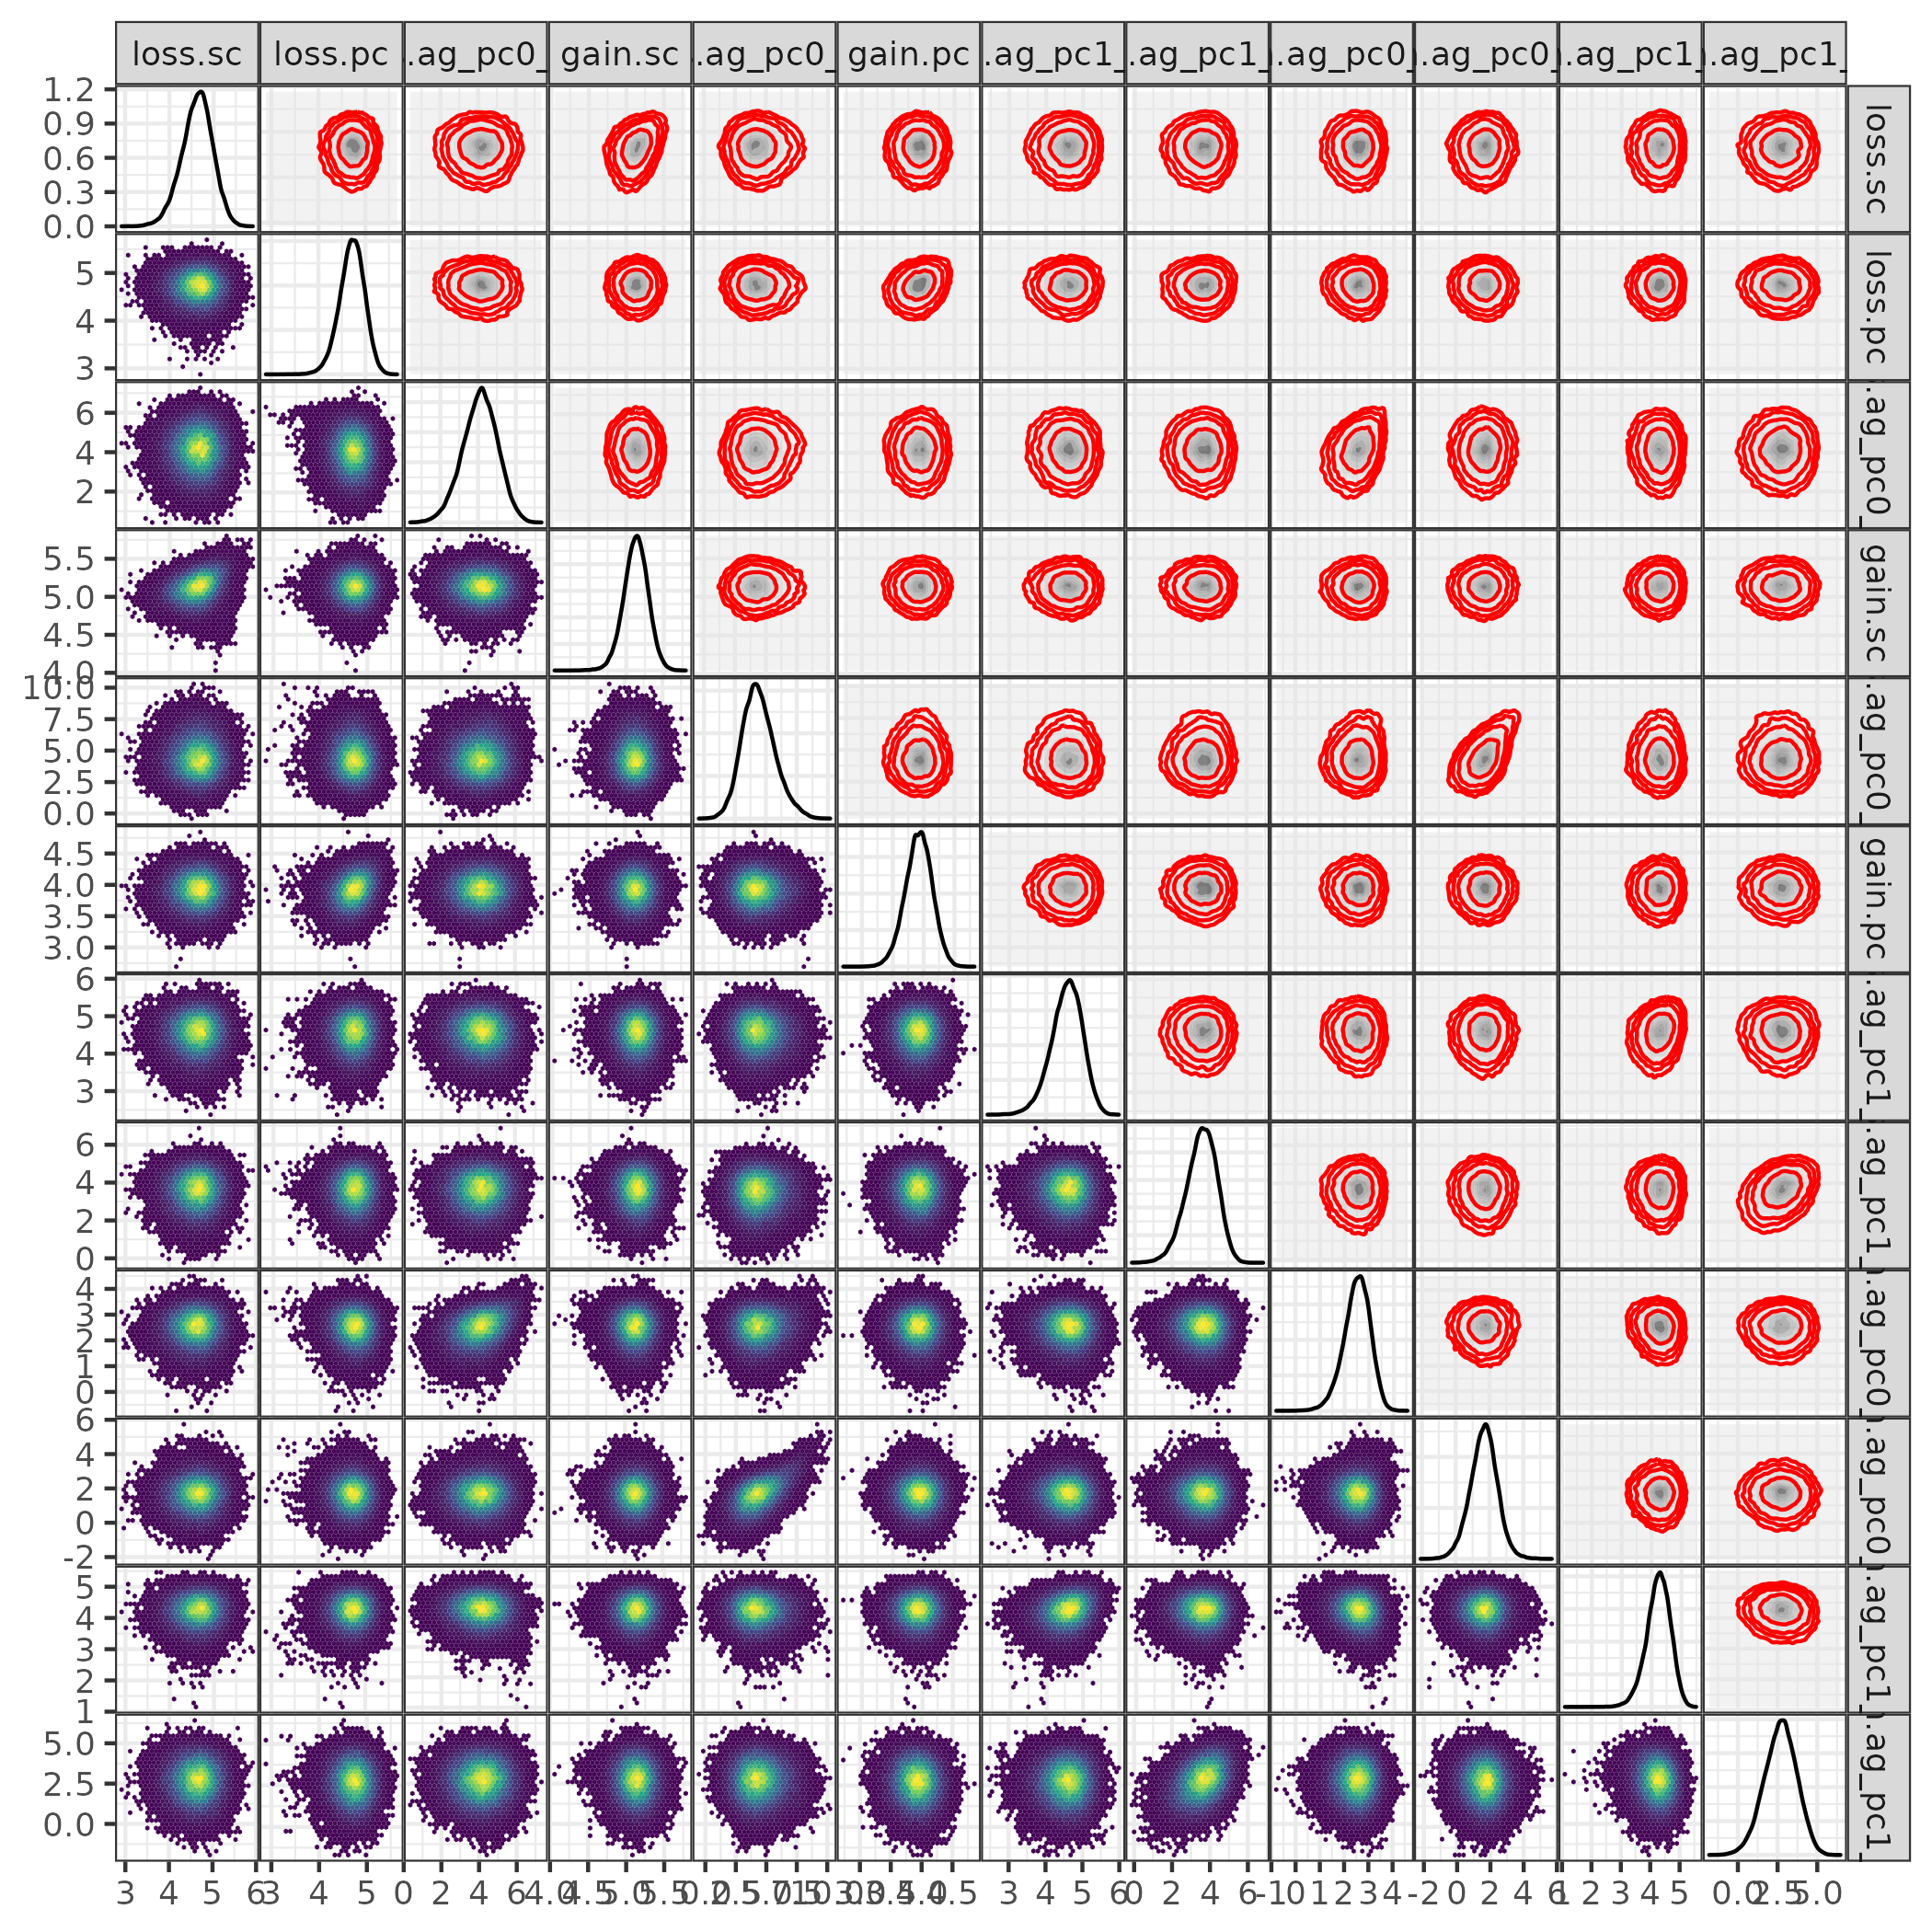
\includegraphics[width=10.5in]{pix/mcmc_pairs_0}

Contour levels are: 50\%, 80\% 90\%, 95\% (largest) highest posterior
density regions.

\hypertarget{treeblock-model-12-parameters}{%
\subsection{Treeblock model (12
parameters)}\label{treeblock-model-12-parameters}}

The model that samples over the `tree block' (sample of phylogeny
reconstructions)

\includegraphics{ag_supp_files/figure-latex/traceplot_tb-1.png}

\begin{verbatim}
## Inference for the input samples (8 chains: each with iter = 8000; warmup = 0):
## 
##                   Q5  Q50  Q95 Mean   SD  Rhat Bulk_ESS Tail_ESS
## loss.sc         4.32 4.89 5.40 4.88 0.33  1.00     9389    17853
## loss.pc         4.45 4.87 5.23 4.86 0.24  1.00    15936    26910
## loss.ag_pc0_sc0 2.45 4.10 5.62 4.07 0.96  1.01     1691     3050
## gain.sc         4.98 5.24 5.48 5.23 0.15  1.00    20255    33733
## loss.ag_pc0_sc1 2.34 4.35 6.81 4.43 1.35  1.01     1147     1838
## gain.pc         3.60 3.97 4.31 3.96 0.22  1.00    17269    30483
## loss.ag_pc1_sc0 4.07 4.76 5.32 4.73 0.38  1.00     8256    14982
## loss.ag_pc1_sc1 2.25 3.69 4.92 3.65 0.81  1.00     1816     4835
## gain.ag_pc0_sc0 1.36 2.41 3.21 2.36 0.57  1.00     3634     7091
## gain.ag_pc0_sc1 0.33 1.69 2.91 1.67 0.79  1.01     2147     2583
## gain.ag_pc1_sc0 4.22 4.81 5.28 4.78 0.33  1.00     9932    11580
## gain.ag_pc1_sc1 1.03 2.76 4.38 2.74 1.01  1.00     2020     4283
## 
## For each parameter, Bulk_ESS and Tail_ESS are crude measures of 
## effective sample size for bulk and tail quantities respectively (an ESS > 100 
## per chain is considered good), and Rhat is the potential scale reduction 
## factor on rank normalized split chains (at convergence, Rhat <= 1.01).
\end{verbatim}

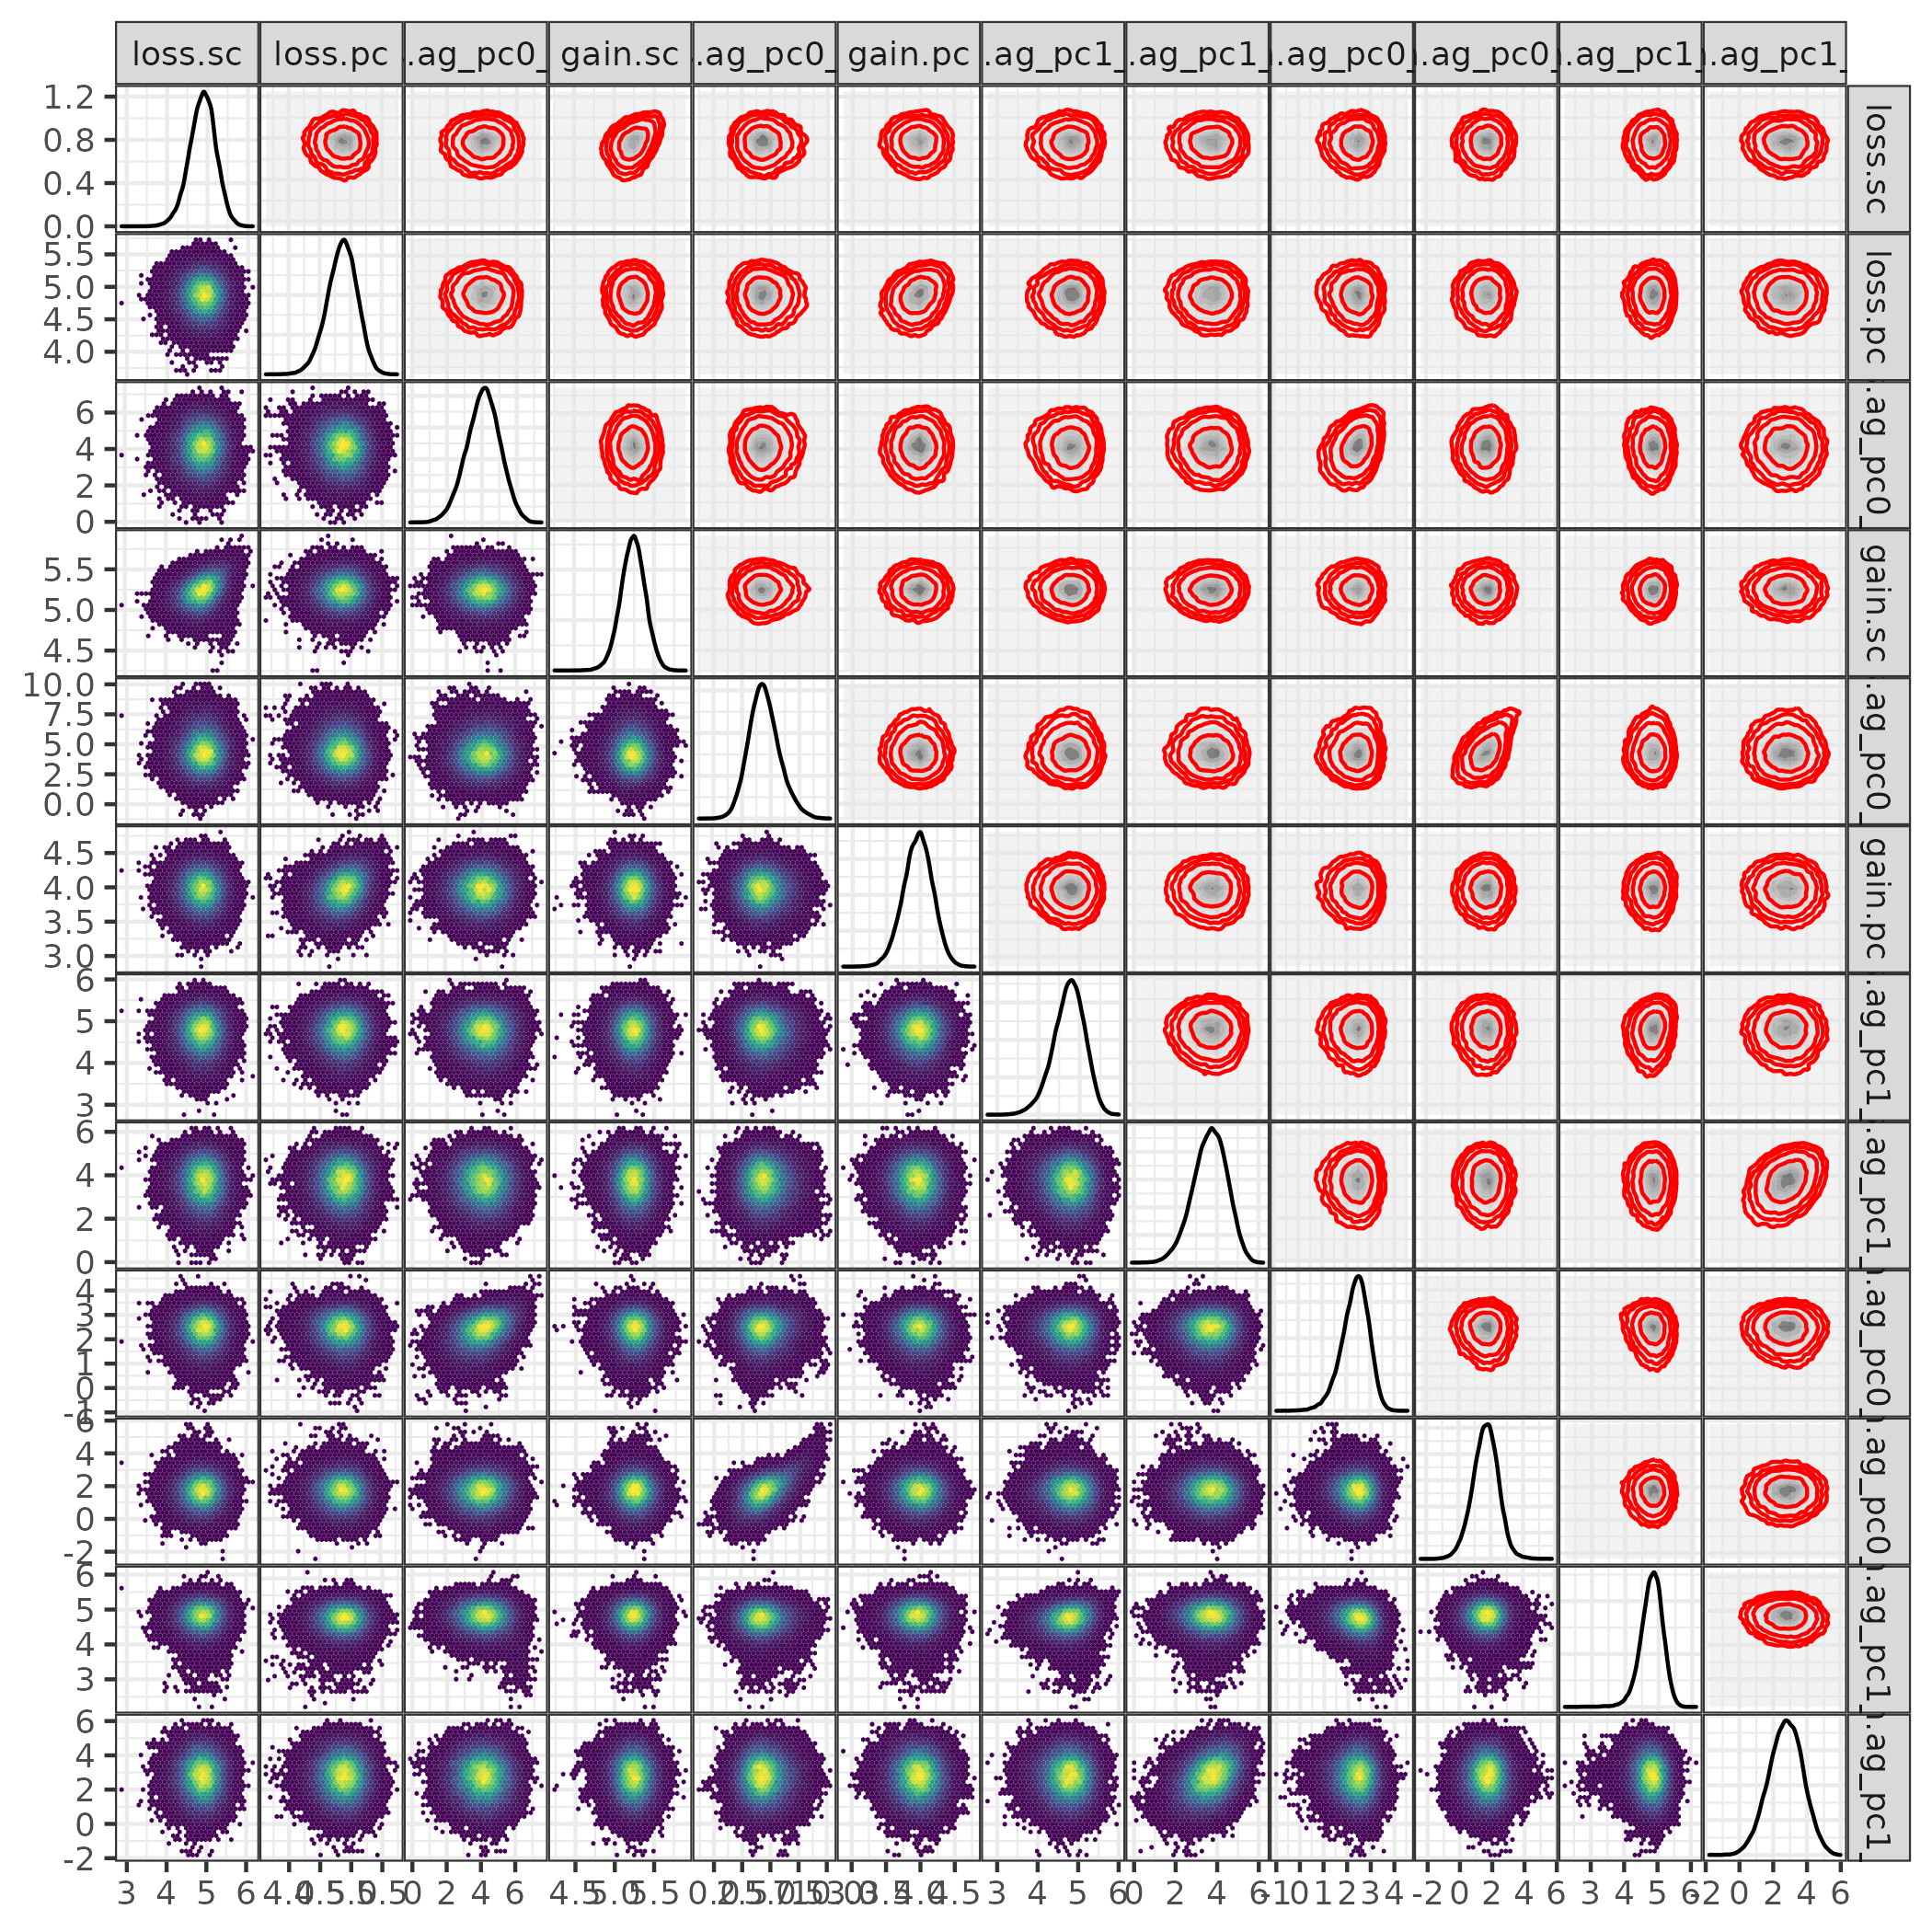
\includegraphics[width=10.5in]{pix/mcmc_pairs_tb}

\hypertarget{full-model-24-parameters}{%
\subsection{Full model (24 parameters)}\label{full-model-24-parameters}}

First half:

\includegraphics{ag_supp_files/figure-latex/traceplot_full1-1.png}

Second half:

\includegraphics{ag_supp_files/figure-latex/traceplot_full2-1.png}

\begin{verbatim}
## Inference for the input samples (8 chains: each with iter = 13600; warmup = 0):
## 
##                    Q5   Q50  Q95  Mean   SD  Rhat Bulk_ESS Tail_ESS
## ag0_pc0_loss.sc  4.00  4.63 5.17  4.61 0.36  1.00    10591    23551
## ag0_loss.pc_sc0  4.22  4.70 5.11  4.68 0.27  1.00    22411    35772
## loss.ag_pc0_sc0  2.47  4.09 5.57  4.06 0.94  1.00     2630     8505
## ag0_pc0_gain.sc  4.82  5.11 5.37  5.10 0.17  1.00    27148    43068
## ag0_loss.pc_sc1  2.42  4.44 7.05  4.55 1.39  1.01     1542     2880
## loss.ag_pc0_sc1  3.48  3.87 4.23  3.86 0.23  1.00    24062    45025
## ag0_gain.pc_sc0  3.83  4.59 5.22  4.56 0.42  1.00    10475    21721
## ag0_pc1_loss.sc  2.07  3.55 4.77  3.50 0.82  1.00     3404     7931
## loss.ag_pc1_sc0  1.36  2.43 3.25  2.38 0.58  1.00     4669    10132
## ag0_gain.pc_sc1  0.34  1.69 2.95  1.68 0.80  1.01     2310     3621
## ag0_pc1_gain.sc  3.38  4.16 4.77  4.13 0.43  1.00    10465    14993
## loss.ag_pc1_sc1  0.89  2.57 4.10  2.54 0.98  1.00     2480     7374
## gain.ag_pc0_sc0 -1.19 -0.09 0.77 -0.13 0.60  1.00     3977     7728
## ag1_pc0_loss.sc  1.96  4.26 6.56  4.26 1.40  1.01     1105     3436
## ag1_loss.pc_sc0  1.92  4.21 6.47  4.20 1.38  1.01     1439     4393
## gain.ag_pc0_sc1  2.02  4.27 6.56  4.28 1.38  1.00      878     2147
## ag1_pc0_gain.sc  1.88  4.26 6.55  4.24 1.42  1.01     1040     2628
## ag1_loss.pc_sc1  1.86  4.18 6.50  4.18 1.41  1.01      918     2721
## gain.ag_pc1_sc0  2.02  4.35 6.58  4.33 1.39  1.01      905     2427
## ag1_gain.pc_sc0  1.79  4.23 6.62  4.22 1.46  1.01      531      892
## ag1_pc1_loss.sc  1.98  4.28 6.59  4.29 1.40  1.00     1129     3046
## gain.ag_pc1_sc1  1.88  4.18 6.44  4.17 1.39  1.00     1609     4535
## ag1_gain.pc_sc1  1.95  4.27 6.65  4.29 1.43  1.01      925     1387
## ag1_pc1_gain.sc  1.92  4.21 6.52  4.21 1.40  1.01     1052     2711
## 
## For each parameter, Bulk_ESS and Tail_ESS are crude measures of 
## effective sample size for bulk and tail quantities respectively (an ESS > 100 
## per chain is considered good), and Rhat is the potential scale reduction 
## factor on rank normalized split chains (at convergence, Rhat <= 1.01).
\end{verbatim}

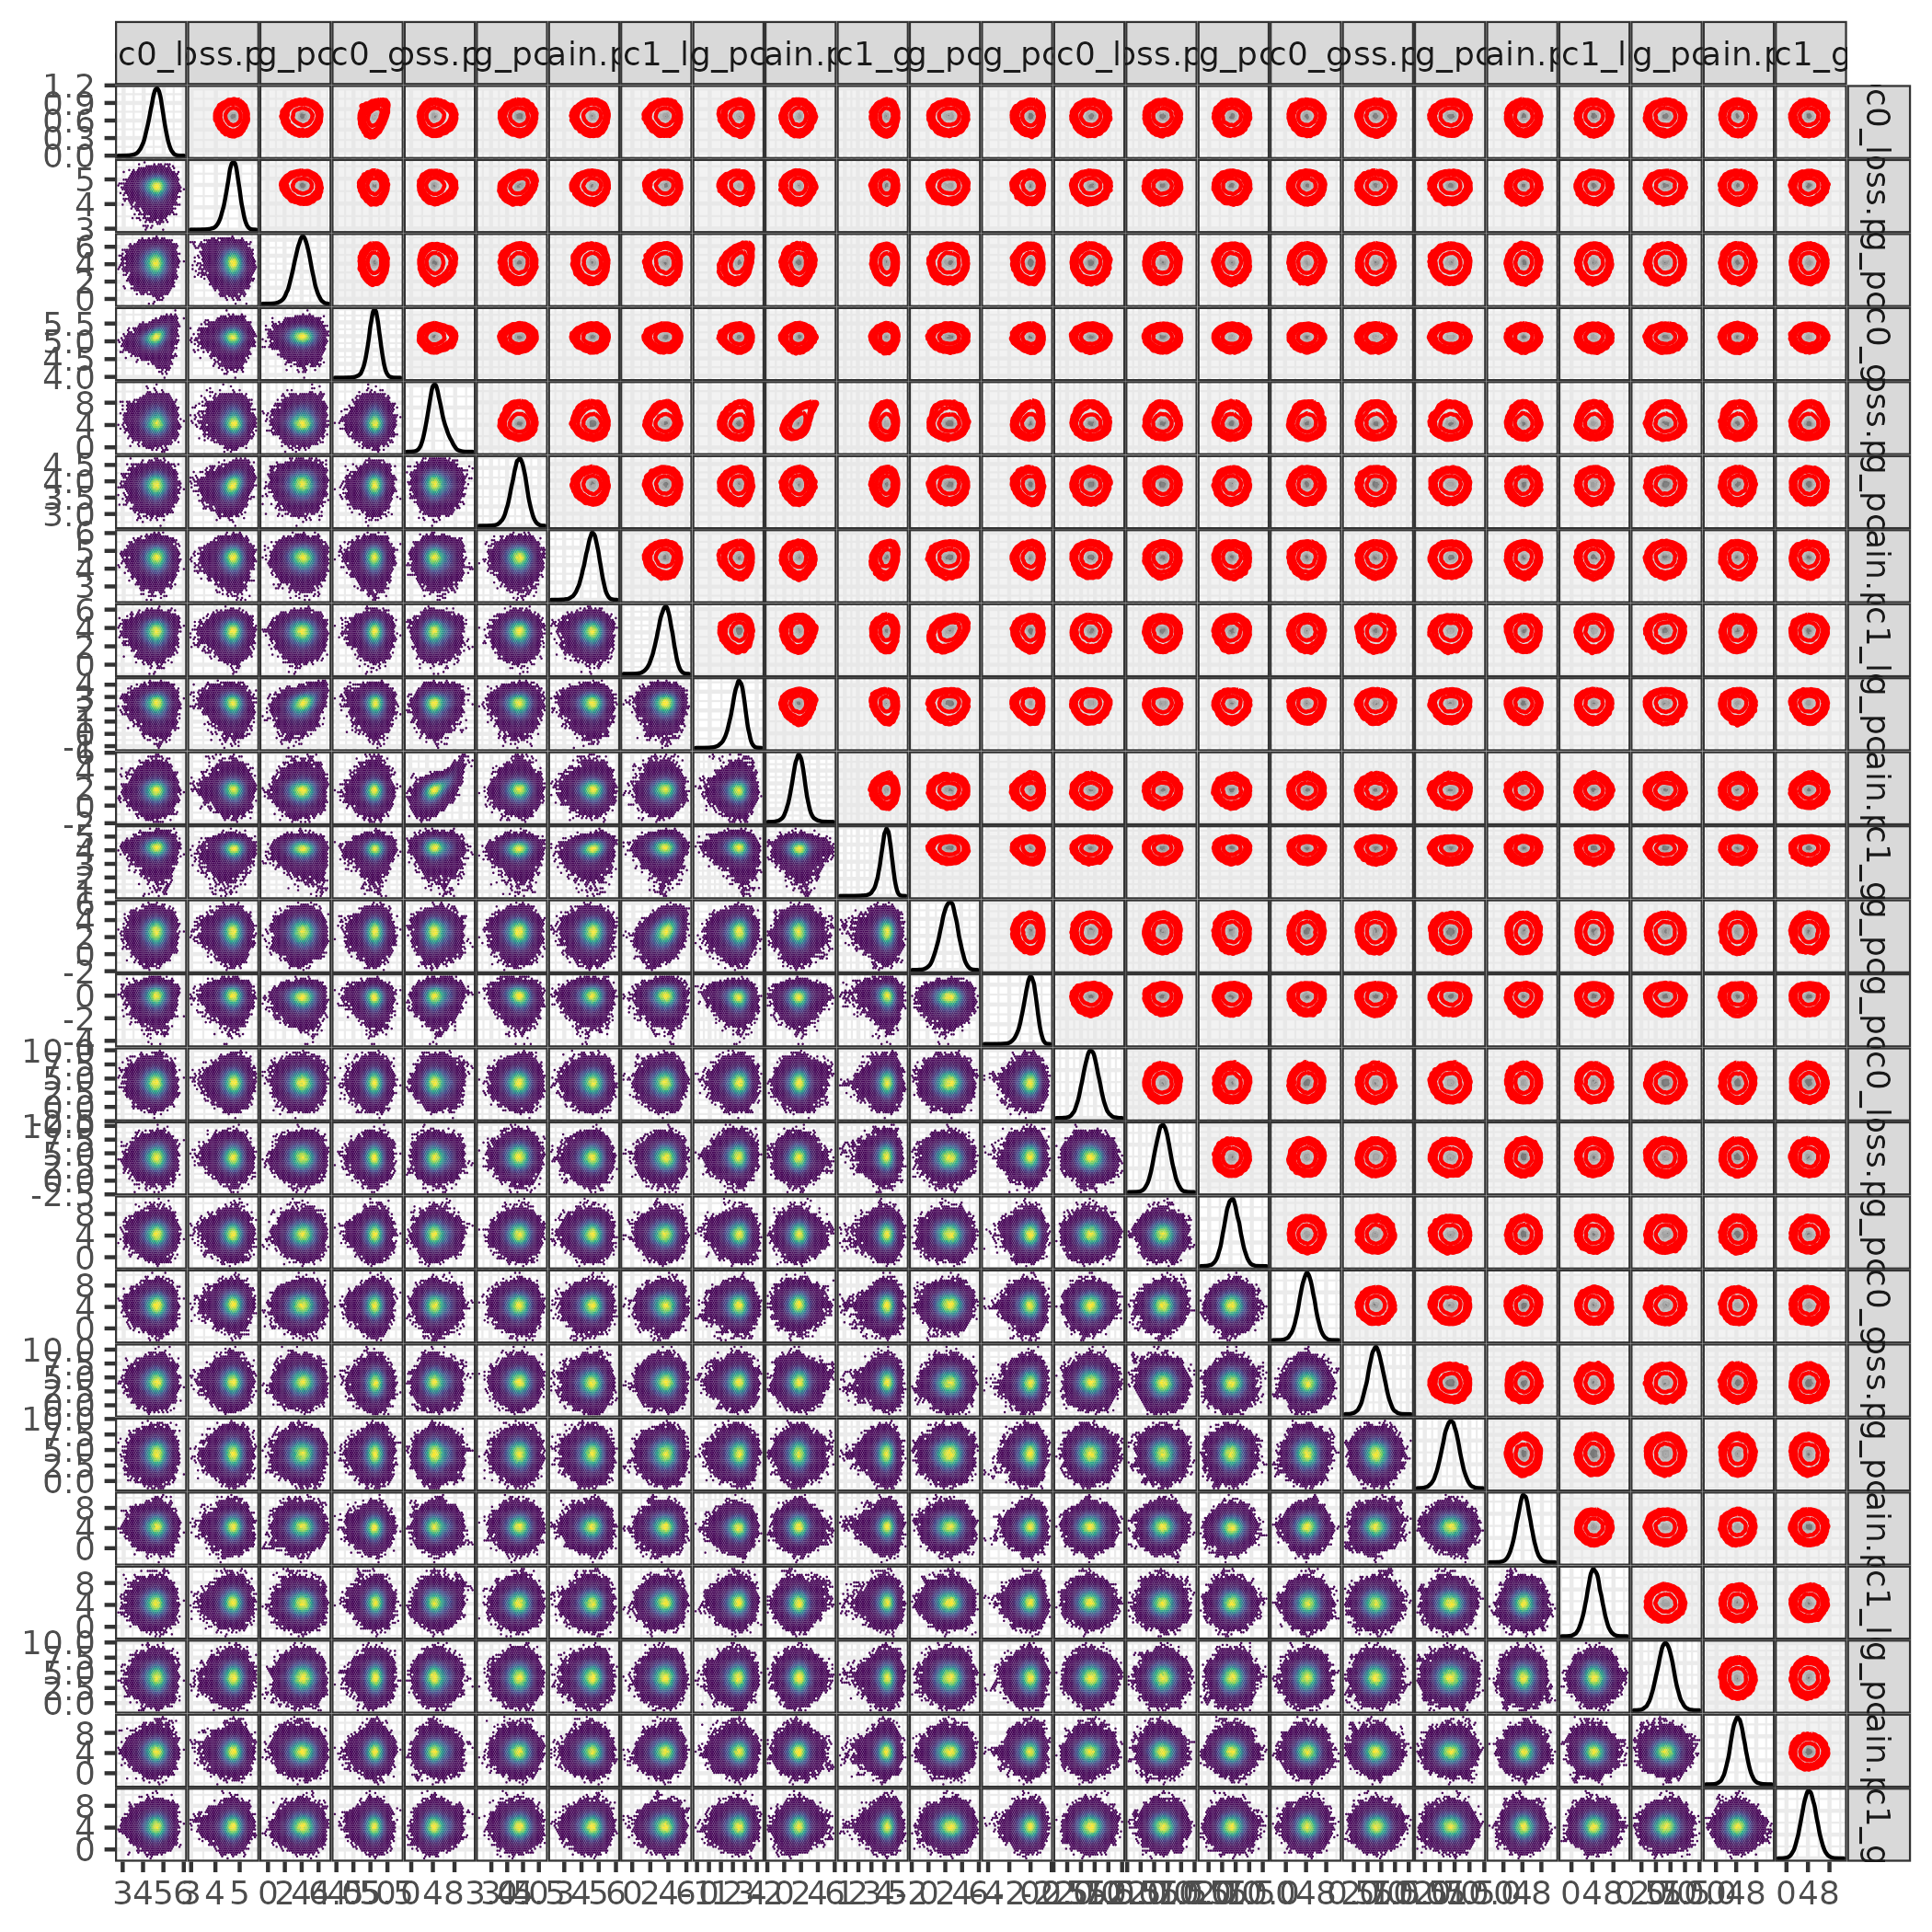
\includegraphics[width=10.5in]{pix/mcmc_pairs_full}

\hypertarget{no-gainloss-priors}{%
\subsection{No gain/loss priors}\label{no-gainloss-priors}}

\includegraphics{ag_supp_files/figure-latex/traceplot_tb_nogainloss-1.png}

\begin{verbatim}
## Inference for the input samples (8 chains: each with iter = 8000; warmup = 0):
## 
##                   Q5  Q50  Q95 Mean   SD  Rhat Bulk_ESS Tail_ESS
## loss.sc         4.19 4.88 5.44 4.86 0.38  1.00     7946    12637
## loss.pc         4.50 4.92 5.29 4.92 0.24  1.00    17867    28501
## loss.ag_pc0_sc0 1.66 3.79 5.54 3.71 1.19  1.01     1147     1783
## gain.sc         4.96 5.23 5.48 5.23 0.16  1.00    18822    21039
## loss.ag_pc0_sc1 2.09 4.94 8.01 5.00 1.79  1.02      679     1864
## gain.pc         3.50 3.90 4.26 3.89 0.23  1.00    18795    31224
## loss.ag_pc1_sc0 3.81 4.61 5.22 4.58 0.44  1.00    11963    16471
## loss.ag_pc1_sc1 1.31 3.18 4.69 3.11 1.03  1.01     1817     2968
## gain.ag_pc0_sc0 1.41 2.47 3.26 2.42 0.57  1.00     5747     8859
## gain.ag_pc0_sc1 0.17 1.69 3.01 1.65 0.87  1.01     1625     2567
## gain.ag_pc1_sc0 4.31 4.87 5.33 4.85 0.32  1.00    14195    22231
## gain.ag_pc1_sc1 1.52 3.49 5.04 3.42 1.08  1.00     1722     3046
## 
## For each parameter, Bulk_ESS and Tail_ESS are crude measures of 
## effective sample size for bulk and tail quantities respectively (an ESS > 100 
## per chain is considered good), and Rhat is the potential scale reduction 
## factor on rank normalized split chains (at convergence, Rhat <= 1.01).
\end{verbatim}

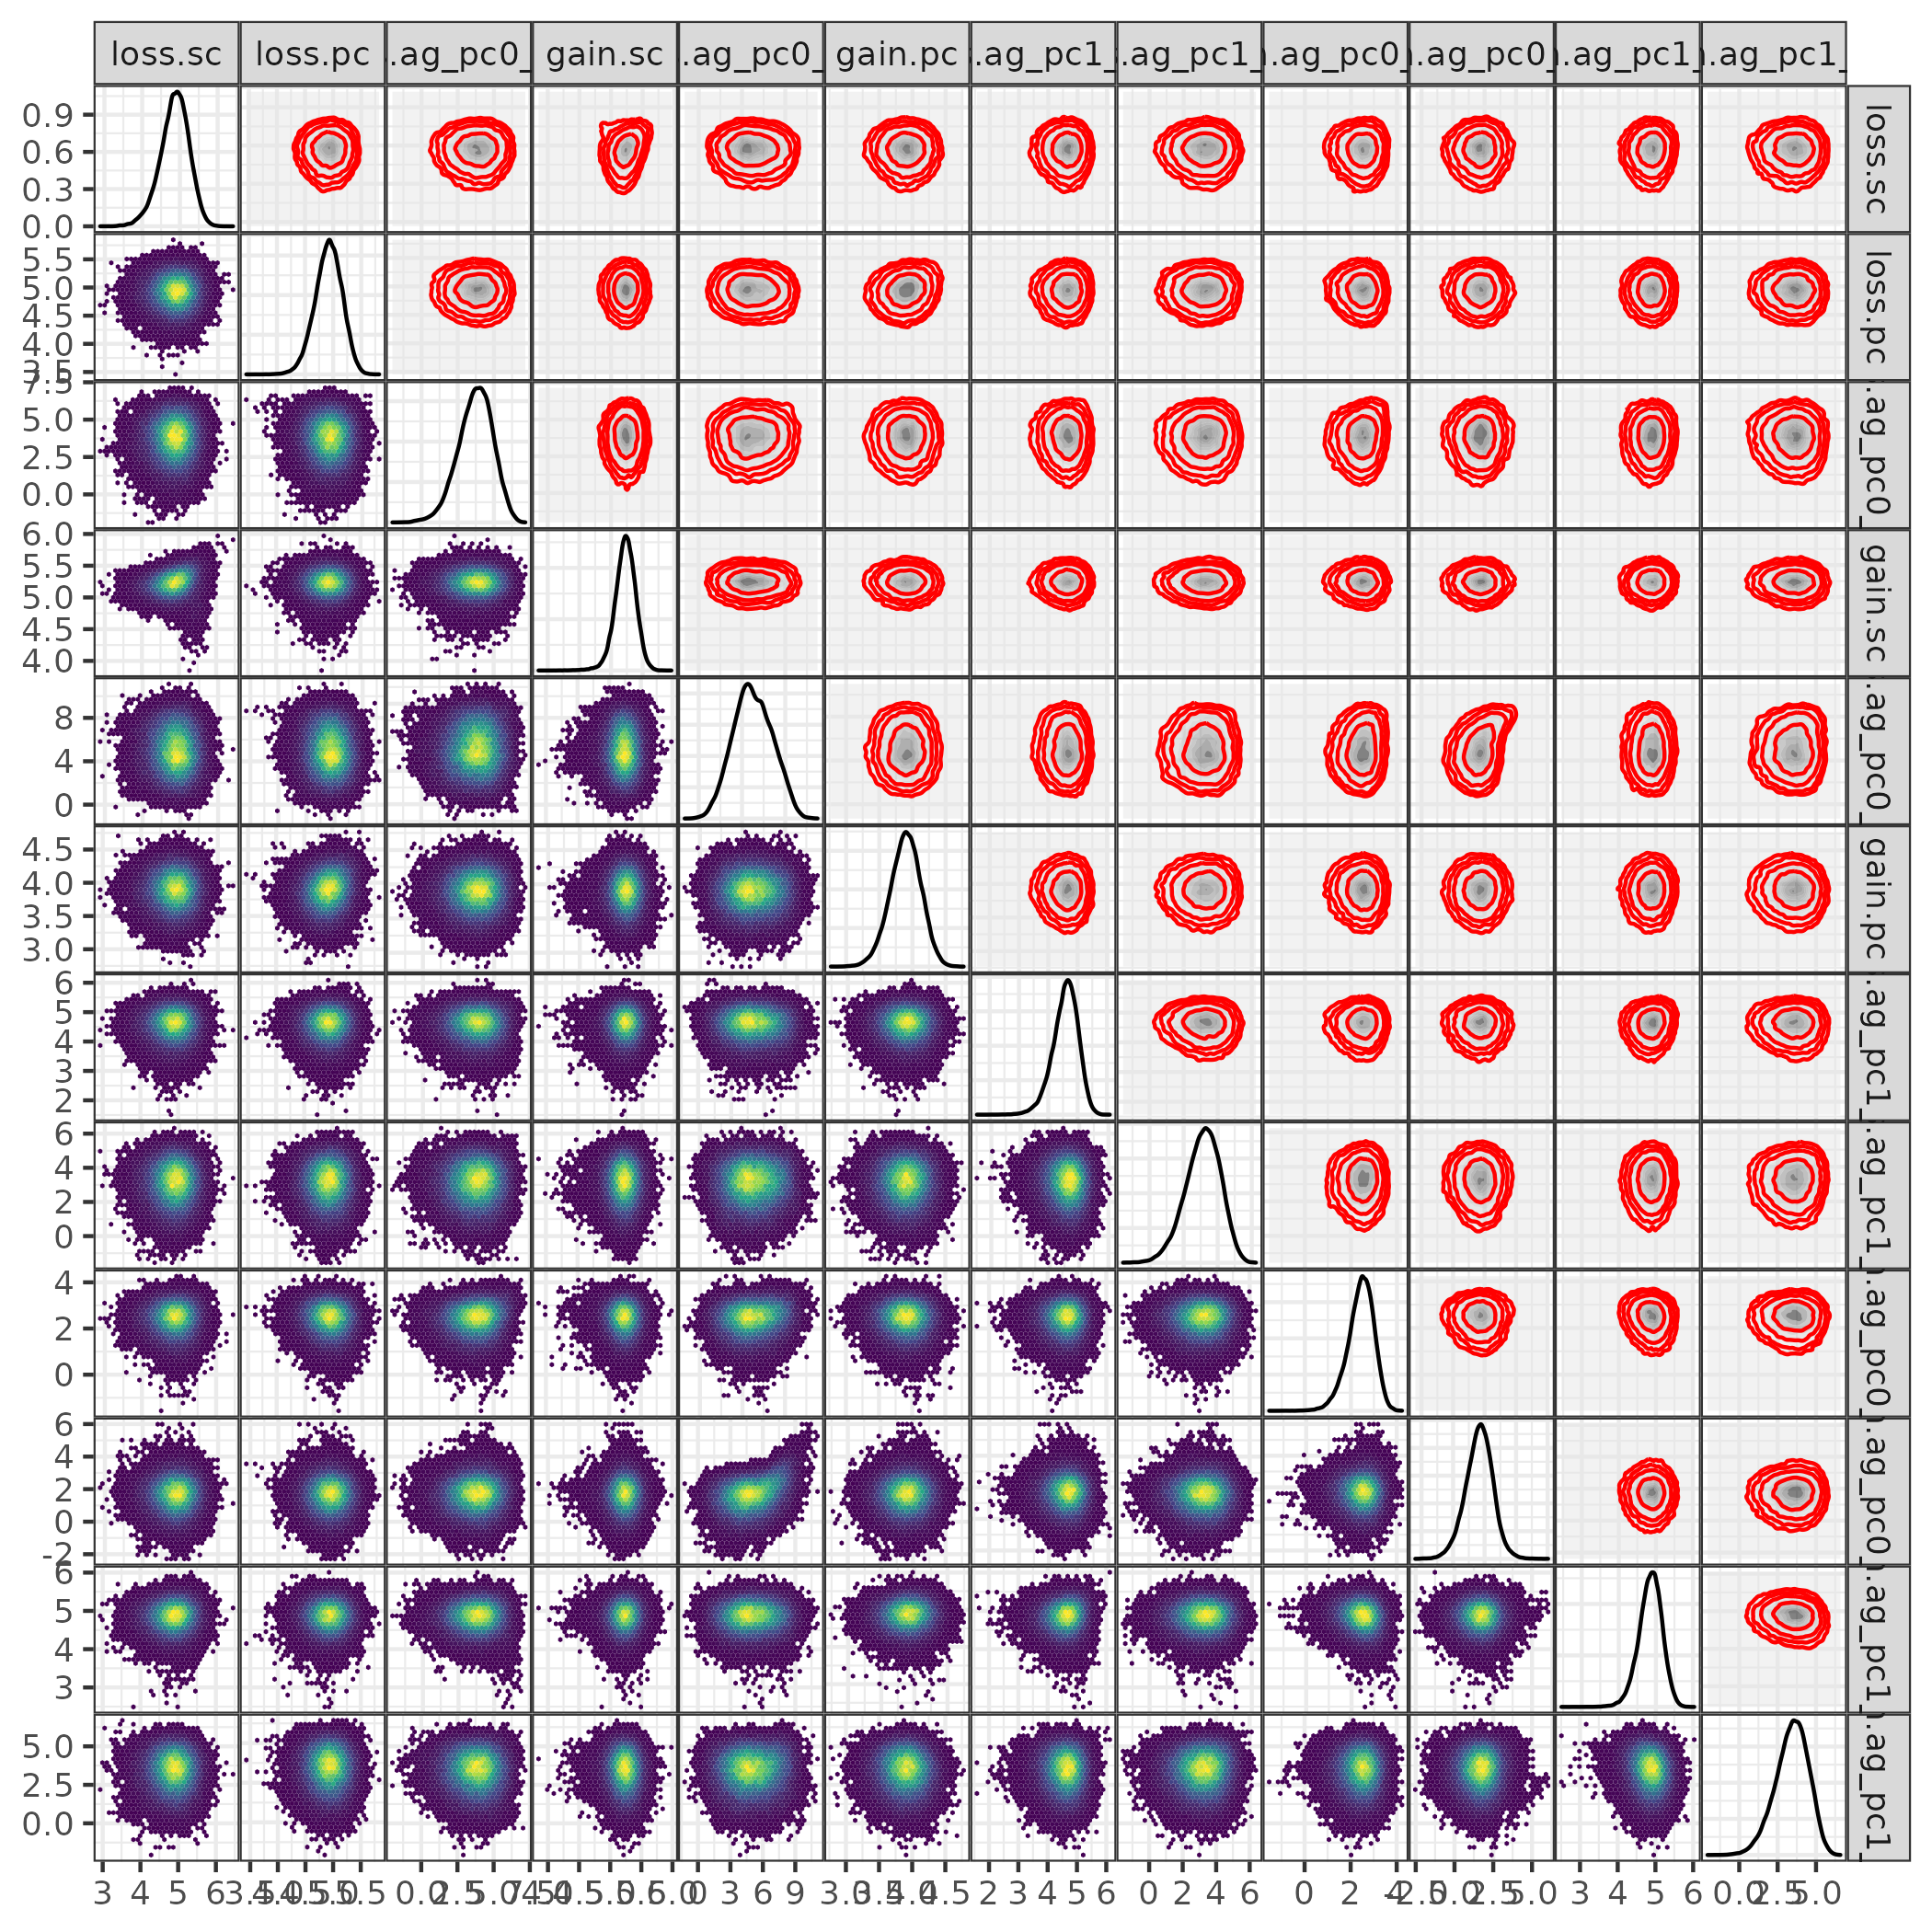
\includegraphics[width=10.5in]{pix/mcmc_pairs_tb_nogainloss}

\hypertarget{references}{%
\section*{References}\label{references}}
\addcontentsline{toc}{section}{References}

\hypertarget{refs}{}
\begin{CSLReferences}{1}{0}
\leavevmode\vadjust pre{\hypertarget{ref-bouckaertDensiTree2010}{}}%
Bouckaert, Remco R. 2010. {``{DensiTree}: Making Sense of Sets of
Phylogenetic Trees.''} \emph{Bioinformatics} 26 (10): 1372--73.
\url{https://doi.org/10.1093/bioinformatics/btq110}.

\leavevmode\vadjust pre{\hypertarget{ref-fox_r_2018}{}}%
Fox, John, and Sanford Weisberg. 2018. \emph{An {R} {Companion} to
{Applied} {Regression}}. 3rd edition. Los Angeles: SAGE Publications,
Inc.

\leavevmode\vadjust pre{\hypertarget{ref-lambertRobust2022}{}}%
Lambert, Ben, and Aki Vehtari. 2022. {``{\(R_\ast\)}: A Robust {MCMC}
Convergence Diagnostic with Uncertainty Using Decision Tree
Classifiers.''} \emph{Bayesian Analysis} 17 (2): 353--79.
\url{https://doi.org/10.1214/20-BA1252}.

\leavevmode\vadjust pre{\hypertarget{ref-makowski_indices_2019}{}}%
Makowski, Dominique, Mattan S. Ben-Shachar, S. H. Annabel Chen, and
Daniel Lüdecke. 2019. {``Indices of {Effect} {Existence} and
{Significance} in the {Bayesian} {Framework}.''} \emph{Frontiers in
Psychology} 10.
\url{https://www.frontiersin.org/articles/10.3389/fpsyg.2019.02767}.

\leavevmode\vadjust pre{\hypertarget{ref-rabosky_inverse_2018}{}}%
Rabosky, Daniel L., Jonathan Chang, Pascal O. Title, Peter F. Cowman,
Lauren Sallan, Matt Friedman, Kristin Kaschner, et al. 2018. {``An
Inverse Latitudinal Gradient in Speciation Rate for Marine Fishes.''}
\emph{Nature} 559 (7714): 392--95.
\url{https://doi.org/10.1038/s41586-018-0273-1}.

\leavevmode\vadjust pre{\hypertarget{ref-shi_reconnecting_2021}{}}%
Shi, Haolun, and Guosheng Yin. 2021. {``Reconnecting p-{Value} and
{Posterior} {Probability} {Under} {One}- and {Two}-{Sided} {Tests}.''}
\emph{The American Statistician} 75 (3): 265--75.
\url{https://doi.org/10.1080/00031305.2020.1717621}.

\end{CSLReferences}

\end{document}
